\subsection{Training the draft: recipe, data, input and size}
\label{app:detail:training}
The main results use one recipe per benchmark (Sec.~\ref{sec:train}). This section varies the recipe
on OpenAGI, where the held-out test set (63 tasks, 263 contexts, scored three times each at temperature
0) is cheap to re-score offline, and then varies the draft size across benchmarks. We split the OpenAGI
test tasks into \emph{seen} (40 tasks whose committed action sequence also occurs in a training task) and
\emph{unseen} (the other 23), because the two respond differently to every knob below.

\begin{table}[t]
\centering
\caption{OpenAGI offline agreement (\%) of 0.6B drafts under recipe variations. Rows marked ``ep\,7''
train for 12 epochs and pick the checkpoint by validation exact match; the Table~\ref{tab:offline} draft
trains for 3 epochs and picks by validation loss (epoch 2). Seen/unseen as defined in the text.}
\label{tab:recipe}
\small
\begin{tabular}{lrrr}
\toprule
draft & overall & seen & unseen \\
\midrule
untrained 0.6B & 12.8 & 11.5 & 14.8 \\
LoRA $r{=}64$, 3 epochs, epoch 2 by validation loss (Table~\ref{tab:offline}) & 75.0 & 82.2 & 64.5 \\
LoRA $r{=}64$, ep\,7 by validation exact match & \textbf{77.1} & \textbf{86.4} & 63.2 \\
LoRA $r{=}64$, epoch 12 & 74.1 & 83.4 & 60.4 \\
full fine-tuning, ep\,7 & 75.2 & 84.7 & 61.0 \\
LoRA $r{=}64$, ep\,7, 50\% of the pairs (535) & 72.0 & 80.5 & 59.4 \\
LoRA $r{=}64$, ep\,7, 25\% of the pairs (270) & 71.5 & 74.7 & \textbf{66.7} \\
\midrule
32B-direct (target, reasoning off) & 76.6 & 76.6 & 76.4 \\
target self-consistency & 97.3 & 98.1 & 96.2 \\
\bottomrule
\end{tabular}
\end{table}

\paragraph{Epochs, capacity and data.}
Table~\ref{tab:recipe} gives the offline agreement. Three findings. (i)~Training longer raises agreement
on seen sequences only: from epoch 2 to epoch 7 the seen score rises from 82.2 to 86.4 while the unseen
score falls from 64.5 to 63.2, and epoch 12 loses on both. (ii)~Full fine-tuning of the 0.6B model does
not beat the rank-64 adapter (75.2 against 77.1). (iii)~Halving or quartering the training pairs lowers
the overall score by five to six points, almost entirely on seen tasks; the unseen score is not monotone in the
amount of data. The two untrained references are flat across the split (32B-direct 76.6/76.4, target
self-consistency 98.1/96.2), so the seen/unseen gap is a property of the trained draft: most of what more
epochs and more data buy is familiarity with training sequences, and the unseen level of 63--67 is not
moved by these knobs. End to end the difference is small. At $k{=}3$ the epoch-7 draft reaches
1.476\xx{} against 1.455\xx{} for the epoch-2 draft, and an independent repeat of the epoch-2 run gave
1.477\xx{}; the live acceptance splits the same way (epoch 2: 82.5\% on seen and 67.0\% on unseen
tasks, 1.53\xx{} and 1.35\xx{}; epoch 7: 86.5\% and 65.0\%, 1.63\xx{} and 1.28\xx{}).

\paragraph{Draft input.}
The draft sees the task and the committed actions. Adding the target's reasoning text for the committed
steps to the draft's input raises the unseen score by at most 2.5 points (64.5 to 67.0, with the epoch-4
checkpoint) at equal overall agreement. In the live runs, however, the draft proposes positions $2..k$ before the
target has produced the reasoning for its own proposals, so training must drop the trailing one or two
thoughts; with that dropout the unseen score falls to 58--60. We therefore keep the action-only input.

\paragraph{Transfer across benchmarks.}
A trained draft is specific to its benchmark (Table~\ref{tab:transfer} in App.~\ref{app:transfer}). On each
of the other three benchmarks, the four trained drafts agree with the target about as often as the untrained
base does, within about four points. The only exception is between the two planning benchmarks: the TaskBench
draft reaches 23.3\% on OpenAGI and the OpenAGI draft 29.6\% on TaskBench, against 13.3\% and 25.3\% for the
base. This is still far below the 75\% of a draft trained on the benchmark itself. Each workload therefore
needs its own draft; training one takes minutes.

\paragraph{Draft size.}
The three drafts of Table~\ref{tab:four} bound the size axis: 0.6B is the smallest base we train and 4B the
largest that shares one H100 with the 32B target at the benchmarks' context lengths. Table~\ref{tab:size} and
Fig.~\ref{fig:size} show what varies. Offline agreement mostly rises with size
(0.6B to 4B: 75.4 to 78.7 on OpenAGI, 74.7 to 80.5 on TaskBench, where 1.7B already reaches 81.0, 63.3 to 69.5 on
$\tau^2$-bench, 66.7 to 79.8 on BFCL), and the draft's cost always does: its per-round term $D$ (Eq.~\ref{eq:S}) grows from 0.16--0.17 to
0.28--0.29 on the planning benchmarks and from 0.03--0.04 to 0.04--0.07 on the tool benchmarks, and sharing
the GPU with the 4B draft raises $\beta$ by up to 0.06. The speedup is the balance of the two. On OpenAGI and
TaskBench, where a target step takes 1--2\,s, 1.7B is the fastest draft (1.55 and 1.47\xx{} against 1.50 and
1.38\xx{} for 0.6B) and 4B falls back to the 0.6B level (1.46 and 1.36\xx{}) although it agrees most; two
independent runs of every cell give the same ordering, and Eq.~\ref{eq:S} predicts it from the sequential
trace (1.48, 1.53, 1.47 on OpenAGI; 1.53, 1.58, 1.53 on TaskBench), with TaskBench
overpredicted by 0.11--0.17. These predictions replay each draft's offline hits using the inputs in
Table~\ref{tab:prediction_inputs}; TaskBench's replayed $\beta$ is 0.05--0.10 below the measured one.
On $\tau^2$-bench, where a target step takes 12\,s and $D$ is 0.03, predicted speedups are 1.58,
1.64 and 1.62; the three drafts measure 1.61, 1.63 and 1.56\xx{}, within one another's bootstrap intervals,
with the 4B draft's calls 1.55\xx{} as long as the 0.6B draft's. On BFCL, where the 0.6B draft agrees least
and a target step takes 11\,s, every size step pays: 1.18, 1.28 and 1.34\xx{} for agreement 66.7, 72.7 and
79.8. The bootstrap intervals of neighbouring cells overlap (OpenAGI 1.7B [1.43, 1.68] against 4B [1.30,
1.62]; BFCL 1.7B [1.20, 1.36] against 4B [1.21, 1.48]), so the ordering rests on its consistency across
runs and benchmarks and on the model rather than on any single pair.

A larger draft pays exactly when its extra agreement outweighs its extra cost, and Eq.~\ref{eq:S} says
where that is: with $c$ the committed steps per round and $\beta + D$ the round cost, draft $B$ beats draft
$A$ when $c_B/c_A > (\beta_B + D_B)/(\beta_A + D_A)$. With the measured values, 4B against 0.6B has a cost
ratio of 1.12 on both planning benchmarks against a gain in $c$ of 1.09--1.10, and on BFCL a cost ratio of
1.03 against a gain of 1.16; on $\tau^2$-bench both ratios are within 0.02 of one, and the three speedups are equal
within noise. The best size therefore depends on the target step. With 1--2\,s steps a mid-size draft is
fastest; with 10--12\,s steps the draft's cost weighs little, and the larger drafts are faster on BFCL and
within noise on $\tau^2$-bench. Training cost grows with size (Table~\ref{tab:size}). The 0.6B draft, trained in
about a minute on OpenAGI, is within 0.1\xx{} of the fastest size in seven of the eight benchmark--target
pairs of Table~\ref{tab:four}, which is why it is our default and the draft of the model validation
(Sec.~\ref{sec:validation}).
For practitioners, we recommend starting with a trained 0.6B draft and $k{=}1$.



\begin{table}[t]
\centering
\caption{\textbf{Draft size.} Three drafts trained with the same recipe. Offline agreement (\%) on the
held-out contexts of Table~\ref{tab:offline}; the measured per-round draft term $D$ of Eq.~\ref{eq:S} in the
common serving configurations of Table~\ref{tab:four}; the speedup Eq.~\ref{eq:S} predicts from the
sequential trace and each draft's own offline hit predictions, with the draft timing sources
listed in Table~\ref{tab:prediction_inputs}. BFCL has no offline-hit prediction (Fig.~\ref{fig:size}).
Measured speedups are in Table~\ref{tab:four}.}
\label{tab:size}
\footnotesize\setlength{\tabcolsep}{3pt}
\resizebox{\linewidth}{!}{%
\resizebox{\linewidth}{!}{%
\begin{tabular}{lrrrrrrrrrrr}
\toprule
 & \multicolumn{4}{c}{offline agreement} & \multicolumn{4}{c}{draft term $D$} & \multicolumn{3}{c}{predicted speedup} \\
\cmidrule(lr){2-5}\cmidrule(lr){6-9}\cmidrule(lr){10-12}
draft & OpenAGI & TaskBench & $\tau^2$-bench & BFCL & OpenAGI & TaskBench & $\tau^2$-bench & BFCL & OpenAGI & TaskBench & $\tau^2$-bench \\
\midrule
0.6B & 75.4 & 74.7 & 63.3 & 66.7 & 0.17 & 0.16 & 0.03 & 0.04 & 1.48\xx{} & 1.53\xx{} & 1.58\xx{} \\
1.7B & 77.6 & \textbf{81.0} & 68.1 & 72.7 & 0.20 & 0.19 & 0.03 & 0.04 & \textbf{1.53\xx{}} & \textbf{1.58\xx{}} & \textbf{1.64\xx{}} \\
4B   & \textbf{78.7} & 80.5 & \textbf{69.5} & \textbf{79.8} & 0.28 & 0.29 & 0.04 & 0.07 & 1.47\xx{} & 1.53\xx{} & 1.62\xx{} \\
\bottomrule
\end{tabular}}}
\end{table}

\paragraph{Objective.}
Sec.~\ref{sec:train} argues that cross-entropy on the target's committed actions is a natural
objective. Table~\ref{tab:objective} lists the comparison that tests alternatives on the two benchmarks with
ground truth, TaskBench and BFCL: supervision from gold labels instead of the target's actions (does the
draft need to imitate the target rather than be correct?) and reinforcement learning from the exact-match
reward starting from the SFT draft. Offline agreement is measured for every variant; the end-to-end speedup
only where the offline gain over SFT exceeds three points; no variant reaches it. On BFCL the gold-label draft is trained with the
same recipe on the benchmark's ground-truth calls replayed in the real environment, one call per decision
(130 tasks, 1{,}200 pairs, 39\% of them turn ends; the target's traces give 1{,}254 pairs, 37\% turn ends).
It reaches 50.5\% decision agreement against 66.7\%: on the 63 held-out decisions where the target calls
a tool it ends the turn 26 times and matches the target's tool group 14 times (22\%), against 3 and
31 (49\%) for the draft trained on the target's own actions; on the 51 single-call decisions alone it matches
14 against 29. Correctness by the benchmark's standard and agreement with the target are different
objectives. The comparison changes the source of the training data, not only its labels: the gold contexts
follow the gold calls, and on BFCL the gold data has one call per decision where the target groups calls.
On TaskBench the gold-label draft reaches 69.9\% against 75.2\%. The gap is smaller there because
the annotated tool sequences often coincide with the target's: they are identical on 61 of the 228 training
tasks and use the same tools, with other argument strings, on 108 more. Reinforcement learning from the exact-match reward, run with GRPO from the SFT draft on the same
1{,}011 training contexts (eight samples per context, reward 1 for the target's action and 0.1 for a call of
the right tool with other arguments, KL to the SFT draft, two epochs, 48 GPU-minutes), raises TaskBench
agreement from 75.2\% to 77.1\%: nine of the 277 held-out contexts change from miss to hit and four from hit
to miss, a net gain that is not significant at this size and that Eq.~\ref{eq:S} values at $+0.04\times$
(replayed $c$ 2.04$\to$2.13), below the three points at which we run the system. The sampled reward on the
training contexts rises from 0.78 to 0.85 while the greedy output changes on 13 contexts, consistent with the reward
sharpening the SFT draft's distribution around actions it already ranks first. Started from the untrained base
instead (25.0\% agreement, 64\% of outputs parsable), the same GRPO reaches 75.9\% after three epochs,
indistinguishable from the SFT draft (12 contexts gained, 10 lost) and 1.2 points below GRPO from it, at
72 GPU-minutes against 4 for SFT: in this setting the reward adds nothing over cross-entropy on the
target's actions, which reaches the same agreement at a fraction of the cost. On BFCL, GRPO from the SFT draft
(reward 1 for the target's exact tool group or turn end, 1{,}254 contexts, two epochs) gains nothing either:
65.7\% decision agreement against 66.7\%, with the exact tool group up from 49.2\% to 50.8\% and turn ends
recalled less often (91.7\% against 97.2\%). This is consistent
with Sec.~\ref{sec:train}: only a proposal made on a prefix the target itself has committed can ever
be committed, so the contexts that decide acceptance are the target's own, and the teacher-forced pairs
already come from them. The tests show no significant gain from GRPO at 12 to 18 times the training cost on
TaskBench; they do not rule out gains from other objectives or larger budgets. An earlier pilot on
other benchmarks found the same one to two points on structured tool use and a loss on open-vocabulary actions.



\subsection{Online training of the draft while the agent runs}
\label{app:detail:online}
The drafts above were trained after a separate collection pass: we ran the target alone over the training
tasks and logged its actions. That pass is not needed. By Proposition~\ref{prop:commit}, every action the
speculative system commits was generated by the target, whatever the draft proposed. So the commits of the
running system are the same supervision, and the draft can be trained from them between batches of tasks.

We test this from a cold start. The untrained 0.6B draft starts the speculative system on the benchmark's
training tasks, in batches (OpenAGI: 250 tasks in 10 batches of 25; $\tau^2$-bench: 60 tasks in 6 batches of 10).
After each batch we train a fresh adapter on all commits so far with the recipe of Table~\ref{tab:recipe},
on a second GPU, and load it into the running draft server without a restart. Batch $b$ therefore runs with
the adapter trained on the batches before it. Each adapter is scored for offline agreement on the held-out
contexts of Table~\ref{tab:offline}, and the final adapter is measured end to end on the test tasks as in
Table~\ref{tab:four}.

\begin{figure}[t]
\centering
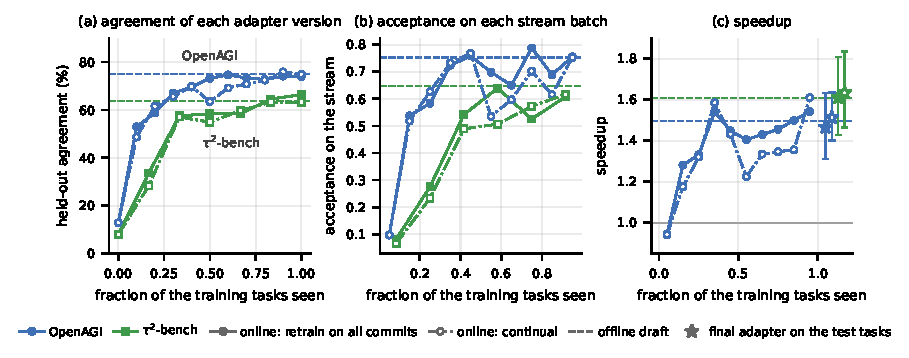
\includegraphics[width=\linewidth]{figures/fig_online_stream.pdf}
\caption{\textbf{Online training of the draft.} The draft is trained online, from the commits of the running
speculative system: the untrained 0.6B draft starts the system on the training tasks, and after every
batch a new adapter replaces the previous one in the draft server without a restart. Colour marks the
benchmark. Solid lines retrain the adapter on all commits so far; dash-dot lines with hollow markers
continue the previous adapter (continual). (a) Offline agreement of each adapter version on the held-out
contexts. (b) Acceptance on each batch of the stream. (c) Speedup on each OpenAGI batch and, as stars with
bootstrap intervals, the final adapters on the test tasks. Dashed: the offline drafts
(Tables~\ref{tab:offline} and~\ref{tab:four}); grey line: no speedup.}
\label{fig:online_stream}
\end{figure}

Figures~\ref{fig:online} and~\ref{fig:online_stream} show the result. On OpenAGI the draft agrees on 53\% of the held-out contexts
after 25 tasks, 67\% after 75, and 74.0\% after all 250 (offline draft: 75.0\%). The speedup on the stream
follows: 0.95\xx{} on the first batch with the untrained draft, 1.28\xx{} on the second, and 1.4--1.5\xx{}
from the fourth batch on. The final adapter gives 1.47\xx{} [1.31, 1.63] on the test tasks, against
1.51\xx{} [1.38, 1.64] for the offline draft under the same serving configuration. On $\tau^2$-bench, with tools executed, agreement on the validation
contexts goes from 8.0\% to 66.4\% (offline draft: 63.7\%), acceptance on the stream reaches the offline
draft's level after 30 tasks, and the final adapter gives 1.61\xx{} [1.43, 1.81] on the test tasks, the same
as the offline draft's 1.61\xx{} [1.44, 1.79]. The buffer ends with 1,079 pairs on OpenAGI, against 1,090 in
the offline training set, because the committed trajectories are the target's own.

Retraining on the whole buffer costs more with every batch (27 to 73 seconds per version on OpenAGI, 3 to
18 minutes on $\tau^2$-bench). A continual variant instead continues the previous adapter on the new batch plus an
equal-size sample of earlier pairs, for two epochs, at a fixed 22 seconds per update on OpenAGI. It reaches
the same endpoint (74.9\% agreement, 1.51\xx{} [1.40, 1.64] on the test tasks) but dips once on the way
(63.5\% and 1.22\xx{} at the fifth batch) before recovering. On $\tau^2$-bench it takes 3 to 6 minutes per update
instead of 3 to 18, ends at 63.3\% agreement (offline draft: 63.7\%), and gives 1.63\xx{} [1.46, 1.83] on the
test tasks. Appendix~\ref{app:online} gives the details.
